% !TeX spellcheck = en_GB
% State-of-the-art text

	Since the main topic of this work, acoustic violent scene detection, has not been researched as such in the literature before, we decided to start our search by addressing close two topics that have been largely studied for the last years related to acoustics scenes and events also including some aspects on violence detection mainly aimed at the detection of violent scenes in movies.
	
\section{\acrlong{asc} and \acrlong{aedc}}

	 \acrfull{asc} refers to the association of an audio sequence to a certain semantic label that describes the environment in which it took place \cite{Barchiesi2015}. With this idea in mind, the classification of acoustic scenarios has been tackled with two different kinds of concepts: soundscape cognition, i.e. understanding how the human being perceives the sounds subjectively from the physical environment that surrounds them  \cite{Dubois2006}, and  \acrfull{casa}, that is working on new computational methods that may help automatize this task through machine learning and processing signal techniques \cite{Wang2006}. This notion can has many applications, such as content recognition --by allowing devices to obtain benefits and information from its situation \cite{Eronen2006}--, for medical usage \cite{Bahoura2009}, as a tool to aid  musical recognition \cite{Van2013} or as a complement to \acrfull{cv}.
	
	Simultaneously to these advances in the \acrshort{asc}, another related area has evolved during the last years: %. Some computational work has been deployed for the tasks of 
	\acrfull{aedc}. It can be described as the processing or treatment of sound signals in order to convert them into significant descriptions that match a listener's sensing of the events and sources composing the acoustic environment \cite{Temko2009}. The detection part consists on identifying the events in a temporal stream of audio and labelling them. The result is usually accompanied by the time interval in which the occurrence is set. However, classification is a task that acts directly on the event that has been already isolated and has the purpose of designating a label or class to the sound \cite{Temko2007}. These techniques also have plenty of applications, e.g., in the medical field \cite{Bahoura2010}, in biological topics such as bird noise detection \cite{Potamitis2014}, and for multimedia information retrieval from video sources in social media \cite{Wang2016}, etc.

	% Version 2 of features and methods
	% !TeX spellcheck = en_GB

\subsection{Features and methods}
	
	As in many fields, the boundaries between features and methods used for audio tasks are becoming blurred since the recent rise of deep learning based methods. Classically, a problem is addressed with a pre-processing stage of the data and then the model or method is implemented. Right now, these two stages are sometimes maintained but also have been mixed or changed depending on how the algorithm used works. In this chapter, we are going to try to explain these difference between features and methods and to separate them in order to ease its understanding.

\subsubsection{Features}

	In every machine learning or pattern recognition task, for the system to be able to infer and extract conclusions from the input given, a pre-processing stage is necessary to make some transformations to the data so that they could be understood by the model. This stage is known as feature extraction and the goal is to convert the original information into a set of values or vectors that characterize the data regarding some desired properties \cite{Giannakopoulos2014}.
	
	There are several ways that allow us to perform this processing stage. The most common and basic one consists on extracting features that are closely related to the original signal which are called \acrfull{lld}  \cite{Amatriain2004}. These are computed by performing some mathematical operations or formulas to the original data and can be considered rudimentary when comparing with other techniques. However, they are really extended and still in use nowadays \cite{Marr1982}. 
	
	\todo{Include small definition short-term features and long-term features? CPM: sí, pero yo lo pondría aquí sino después de la tabla. Algo así como: Moreover, the temporal and spectral features can be further classified as short or long-term...}
	In the audio field, there are two types in which all \acrshort{lld} can be grouped into. One of them is for the features that have been computed by considering the audio signal in its original form in the recording, i.e., in time-domain, that is the reason why they are known as time-domain audio features. The other case refers to those characteristics that are obtained from the signal after having been transformed into the frequency domain. These are commonly known as frequency-domain or spectral audio features. For the procedure of feature extraction, the signal is usually divided into frames that can be overlapped by using a sliding window, so the calculations are done per frame, obtaining a final matrix with size $number\ of\ frames \times number\ of\ features$ \cite{Giannakopoulos2014}. It must be taken into account that the goal of the whole system is going to be fundamental at the time of deciding which features must be computed. For example, not the same features are to be used for speech recognition than for musical information retrieval. In table \ref{table:6}, a summary of most used time and spectral features is included.
	
	% Table of time domain features
	\begin{table}[h!]
		\begin{center}
			\centering
			\begin{tabular}{|| m{9em} | m{24em} ||}
				\hline
				\begin{center}\textbf{Feature}\end{center}& \begin{center}\textbf{Description}\end{center} \\
				\hline\hline
				\multicolumn{2}{||c||}{\textbf{Time}} \\
				\hline
				Energy Entropy & It is useful to detect sudden changes from the energy of a signal. To calculate this value for a certain subframe, it is necessary to first compute the normalized energy of the subframe with respect to all the frames energy \cite{Giannakopoulos2006}. \\
				\hline
				Short time energy & It is the energy for a short segment of signal. It is normally used in speech-related tasks in order to identify voiced form non-voiced fragments \cite{Garcia-Gomez2016}, among other things. \\
				\hline
				\acrfull{zcr} & This can be defined as the number of times the amplitude of the signal crosses the zero line per unit of time, i.e., changes from negative to positive. It is sometimes computed by the number of zero-crossings by the amount of samples in the frame \cite{Giannakopoulos2006}. \\
				\hline
				\multicolumn{2}{||c||}{\textbf{Frequency}} \\
				\hline
				\acrfull{sf} & It is computed to measure the spectral changes between two successive frames. To do so, the difference of their normalized squared spectra coefficients  \cite{Giannakopoulos2006}. \textcolor{red}{CPM: pero no dices respecto a qué está normalizado} \\
				\hline
				Spectral Rolloff & This represents the skewness of the shape of the spectrum given the frequency below which a concrete percentage of the magnitude distribution of the frequency transform is concentrated \cite{Garcia-Gomez2016}. \\
				\hline
				\acrfull{sc} & This is a measure related to the spectral position. It is defined as the center of gravity of the spectrum. %, i.e., \doubt{it indicates how high the spectrum values are on average} 
				\cite{Giannakopoulos2006}. \\
				\hline
				\acrshort{mfcc} & It is a feature that it is widely used because it gives good results in many tasks as for example, speech recognition since it interprets the frequency bands in a very similar way to human perception while doing a separation of the fine structure of the spectra (that corresponding with the harmonics) and the coarse (i.e. the filter representing the vocal tract). It is computed from the \acrshort{stft}.\cite{Garcia-Gomez2016}. \doubt{A detailed explanation can be found in appendix \ref{}}. \\
				\hline
			\end{tabular}
		\end{center}
		\caption{Examples of time  and spectral audio features.}
		\label{table:6}
	\end{table}

	Then, a typical procedure would first divide the signal into frames and performed the desired mathematical and statistical transformations to obtain a \acrshort{lld} vector per sample in order to pass these input data to a statistical model that will be trained with the objective of summarizing the properties of the signals and develop a classification rule so as to be able to assign a faithful category to a new unlabelled observation \cite{Stowell2015}.
	
	In some cases, the mentioned descriptors, sometimes referred as manually-crafted features, are not enough to model data since they cannot achieve a meaningful enough representation of the original information for the system to learn from. Also, as mentioned above, the selection process of this type of features plays a significant role in the final output so that the criteria of the designer could be considered a limitation for the classification task \cite{Grill2012}. For this reason, a new strategy of addressing feature extraction has appeared based on the idea of finding more specialized properties by using specific engineering algorithms that explores the given data in order to find non-human recognizable patterns. The techniques that allow to perform this task are usually called automated feature generation algorithms or machine-learnt features \cite{Pachet2009}.
	
	In order to compute these high-level features, there is not just one standardized machine model that allow to compute them all in a particular form. The calculation method, nevertheless, differs from one approach to another. One example could be the combination of low-level data with high-level semantic descriptors that consists on the inference of diverse musical dimensions by using support vector machines so as to find similarities among music genres. Particularly, they consider the output probabilities of the \acrshort{svm} classifier as a high-level feature space in which the distance between samples from different classes can be measured \cite{Bogdanov2011}. Some other application example could be building high-level feature detectors for image recognition by using unlabelled data to feed a \acrfull{nn} model \cite{Le2013}. 
	
	\todo{CPM: aquí hace falta que pongas ejemplos de feature extraction en AED. Basta un párrafo con dos o tres refs. Si no, no se sabe qué relación tiene esto con nuestro problema y cual es el estado del arte en nuestro problema en particular. Creo que todo esto lo tienes en el Features and Methods antiguo que ahora voy a leer. Creo que deberías cambiar el título de la sección 2.1.1 por 2.2 Features and methods for ASC and AED/C y complementarlo con las de la sección 2.1.2}
	
\subsubsection{Classification models}
	
	Several algorithms have been designed in order to perform a classification task by finding patterns from input data features. Next we will present briefly some of the most commonly used in the literature and then provide a more detailed description of those we have used in this project. In particular, the most basic methods to tackle the classification task are \acrshort{knn}, \acrshort{svm} and also \acrshort{gmm} \cite{Fu2011}.
	
	In the case of \acrfull{knn}, given a set of samples ${x_1, ..., x_n}$ that belong to a metric space $X$ whose labels are ${\theta_1, ..., \theta_n}$ respectively, if a new sample $x$ comes in, it will be categorized by following a majority vote process of the nearest neighbours considering a distance in the space $X$. A trade-off must exist in the choice of the number of nearest neighbours since on the one hand, it is desirable for it to be large so that the voting process has more participants and  the probability of misclassification is minimized and on the other, a small value with respect to the total number of samples so the nearest points are close enough to the new observation \cite{Cover1967}. \todo{Complete with example in the ASC or AEDC approaches. CPM: ok. Do not forget about it.}
	
	 \acrfull{gmm} are a class of soft clustering methods. They are commonly used to derive global statistical properties from the feature vectors of the sample data. Specifically, considering $K$ clusters, they define a group of feature vectors from training data belonging to a certain category $q$ and model them as a multivariate normal distribution $N(\mu_k, \Sigma_k)$ that is further weighted by the probability $w_k$ of a particular of a certain observation to belong to cluster $k$. After learning a global model for the training data $M_q={w_k, \mu_k, \Sigma_k}$, a new observation will be categorized by applying the maximum likelihood criterion \cite{Stowell2015}. \todo{CPM: ok pero, ¿sabes qué estás diciendo si te preguntan?}
	
	However, the one that has been generally more successful is the \acrfull{svm} classifier \todo{CPM: pero esto será cierto en un determinado campo, ¿no? Yo no sería tan rotunda diciendo esto salvo que pongas una cita apoyándolo o lo delimites a un campo en particular.}. There are plenty of works in the literature that use this technique for audio classification tasks \cite{Jiang2005} \cite{Geiger2013} \cite{Barchiesi2015}. It is originally known to be a binary classifier but, nowadays, there have been some implementations that allow its use it in multiclass problems. This algorithm makes the classification by taking into account pairs of observations that are more likely to be misclassified and draws a hyperplane as the optimal boundary between the two classes \cite{Fu2011}. Since this technique has been used for the experiments in this work, a more detailed explanation will be included in section \ref{section:models}.
	
	Finally, we should mention all the techniques or algorithms that have been developed based under the idea of \acrfull{ann}. This concept was inspired by human biology and how the neurons communicate among them in the brain in order to interpret the input or sensory data humans collect. 
	
	\todo{CPM: yo acabaría este apartado aquí y volvería a decir (en el párrafo anterior) que las ANN se explicarán en 3.4. Lo que viene es demasiado detallado y demasiado alejado de ASC como para estar en el estado del arte. }
	
	The \acrshort{ann} intention is exactly to transform input data into a desired output so that it performs a given task. %it can understandable by a machine. 
	A basic architecture is usually composed by an \textit{input layer} of neurons, a certain number of \textit{hidden layers} and an \textit{output layer}. The model receives some input, typically a feature vector, and pass it trough the hidden layers in order to perform some transformations. The neurons of a layer are completely connected to the neurons of the next layer but neurons in the same layer are not usually connected. For this case, we can say that they are \acrfull{fc} layers. Finally, the output layer gives the final outcome of the network \cite{Kwon2011}. This is just the basic and initial nature of the idea but it was implemented in many different ways depending on the input data and the desired task.
	
	\todo{Include image of FCC? CPM: ¿FCC? Do you mean FC or a DNN? It could be a good idea }
	


	
	
	
	

	
	
	
	
	
	
	
	

\subsection{Features and methods}
\label{subsection:features-and-methods}
	
	In the literature, numerous articles have been published related to \acrshort{asc} field. These can be sorted into two different trends based on how the problem is addressed. One of them considers the scene as a single instance with the purpose of representing it through a long-term statistical distribution that models a set of low-level features \cite{Stowell2015}. An acoustic event can be characterized in different ways for this type of method. In previous works, feature extraction methods imported from the field of speech recognition played a main role in this field too, such as the \acrfull{f0}, the \acrshort{f0} envelope and the probability of voicing. Apart from these, also spectral features, as Mel-Spectrum bins, \acrfull{zcr} and \acrfull{sf}, and energy features, such as the energy in bands or the logarithmic-energy \cite{Geiger2013} had an important function on this task. However, the best results have been achieved with the so-called  \acrfull{mfcc}, defined as a cepstral feature\todo{Explain more MFCC? CPM: acuérdate de esto.}, \doubt{which will be explained further on. CPM: sí, referencia dónde lo has puesto}. This kind of characteristics extracted from the audio can be called low-level descriptors and they are usually combined with algorithms and methods to address the classification task. In this "bag-of-frames" approach, in which the scene is considered as a single object, a typical technique was to model the samples features into global statistical characteristics from the local descriptors by using \acrfull{gmm} \cite{Aucouturier2007}. \todo{CPM: aquí hay cosas redundantes con la sección 2.1.1 que te propongo que se transforme en 2.2}
	
	There is another path to dig for \acrlong{asc}, which consists on including a representation of data prior to the classification, which transforms the scene by using a set of high level features normally obtained with a vocabulary or dictionary formed by acoustic atoms. These are usually a depiction of events or streams within the scene and do not need to be known a priori \cite{Stowell2015}. Apart from the typical well-known audio features, the ones named above as low-level descriptors, there exists other acoustic characteristics which may seem to be hidden in the data but can be found by using unsupervised-learning methods. This is the way to act when dealing with the above mentioned acoustic atoms. 
	
	One of the approaches that can be found in the literature about this idea is based on the use of a previously learned over-complete dictionary that is utilized to sparsely decompose the spectrogram of audio. This dictionary will be used by an encoder with the purpose of mapping new input data to real similar versions of their own sparse representation in a fast and efficient way. Finally, the obtained codes will feed a \acrfull{svm} classifier, used for the task of music genre prediction \cite{Henaff2011}. \todo{Include results? CPM: no, porque son de otro campo. }
	
	Another job done in the sparse-feature representation framework presents a way of mixing high feature learning techniques with a pooling method for the objective of music information retrieval and annotation. After some preprocessing of the audio signals data, three feature-learning algorithms are trained finding that sparse restricted Boltzmann machine (sparse-RBM) gets better results than K-means and Sparse Coding. Once the features are obtained, an extra step takes place before performing the classification task, the one called pooling and aggregation. The goal of this procedure is to achieve a feature representation for a long sequence such as a song. Since when joining short-term features that belong to small segments inside the song may result in a loss of their local meaning, a max-pooling operation is computed over each subsegment in order to just consider the maximum value for each feature dimension. After that, these are aggregated by computing the average. The max-pooling contribution resides on reducing the smoothing effect when averaging the values \cite{Nam2012}. This approach is feasible because of the homogeneity in music data. However, this technique could be slightly risky when dealing with acoustic scenes. For this case, a modified version of this method has been proposed. Taking into account that the presence of events is less frequent, instead of considering the whole long sequence to apply the max-pooling for, it will just be used in those segments that had been already detected as significant events by establishing a threshold value and setting an onset and offset that allow to know the start and end time \cite{Lee2013}. \doubt{The representation of the audio event  in a feature space explained in this case is the one that better fits our approach (\ref{section:our-approach}) until now.}
	\todo{Include picture of the pipeline? CPM: pero aquí no. Si lo haces, en el capítulo de Methods y aquí dices en qué sección lo desarrollas.}
	
	The classification of acoustic scenes can be linked to event detection. The working method used for this task is really similar to the one used for \acrshort{asc}. Thus, it is not surprising that most of the works found in the literature address this task with the use of \acrshort{mfcc} as features and with techniques such as \acrshort{hmm} or \acrshort{gmm}. For the purpose of finding the desired events, the whole detection process can be split into two parts. Firstly, a classification of already isolated events should be executed in order to build a vocabulary of acoustic actions. In this case, the data used belong to short-term sequences that must strongly show the semantic meaning of the corresponding event. This is important because there may be more acoustic representations in the same short segment than the one to be detected, but this must stand out among the others.  Consecutively, for the detection part, the input data will be composed by long tracks so that time allocation of the events will be implemented. Therefore, after obtaining the different short segments from dividing the long sequence up, they will be classified considering the results from the first step \cite{Mesaros2010}. \todo{Go deeper? HMM, GMM, MFCC}
	
	A novel type of feature has been used in the last years that differs from the already explained low-level and high-level ones: \acrfull{dnn} have grown increasingly for plenty of classification tasks and so in the multimedia area. The problem with this type of systems is the huge amount of data that is needed to make them work properly, which can be translated in a lack of labelled data. One of the habits that has been currently resorted by the researchers consists of learning what is called deep data \textit{embeddings} from extensive collections of, ir our case, audio and use them so as to perform \doubt{shallow classifications by using simpler datasets}. There have been implemented some models about this topic, such as \acrfull{l3} \cite{Cramer2019} net that uses as input for the the embedding extractor the linear-frequency log-magnitude spectrogram of 60 million audio samples, the system called SoundNet \cite{Aytar2016} that has been designed to obtain embeddings from training a deep audio classifier in order to predict the output o a deep image classifier and the \acrshort{vgg}ish network, designed by Google researchers. This last case is the one we used in this work and it will be explained in more detail in section \ref{section:feature-extractor}. \todo{CPM: esto está muy bien.}
	
\subsection{Transfer learning}
\label{subsection:transfer-learning}

	All these models previously mentioned allow us to use complex extractors trained with huge collections of data and apply them to models considerably much less complicated to address other type of problems. This is possible due to a kind of techniques commonly known as transfer learning and domain adaptation.
	
	The typical consideration in plenty of machine learning tasks consists on extracting the training and testing subsets of data from the same feature space and same distribution. When one of these initial assumptions change, it is necessary to rebuild the whole model from the initial point, including new training data, which means a lot of computational cost and loss of efficiency \cite{Pan2010}. Its working manner can be explained as an analogy of how humans transforms their ability on a certain task to obtain knowledge for other purpose. An example could be how musicians apply their previous experience to get to know faster how to play another instrument.
	
	The first work in which this topic has been treated widely was in 1995 in the workshop \textit{Learning to Learn} \cite{Sarkar2018} and since then many approaches have arisen and renamed the same idea as knowledge consolidation or inductive transfer. However, it was 10 ten years later, in 2005, when the first idea of the ability of a system to identify and apply learned skills previously to completely new problems appeared from the hand of the \acrfull{baa} 05-29 of \acrfull{darpa}’s \acrfull{ipto} \cite{Pan2010}. This can be expressed as a relation between a \textit{source} task, where the abilities are learned, and \textit{target} task, the novel problem that needs to be resolved. As a difference with other similar methods, in this concept of transfer learning the roles of these two are not equal since the weight of the target is much heavier. In figure \ref{fig:mesh4} it is shown the difference between a common machine learning approach and the use of transfer learning.
	
	% Difference between machine learning and transfer learning
	\begin{figure}[h]
		\centering
		\captionsetup{justification=centering}
		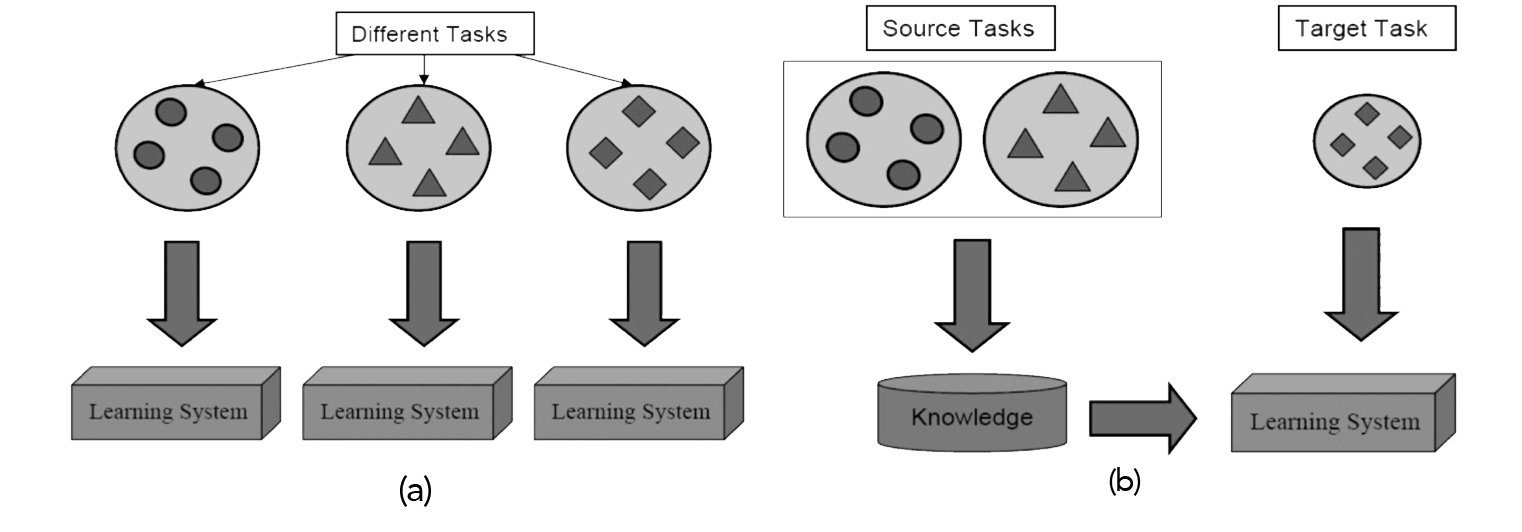
\includegraphics[width=0.8\linewidth]{ml_tl}
		\caption{Difference between traditional machine learning (a) process and feature learning (b) \cite{Pan2010}}
		\label{fig:mesh4}
	\end{figure}
	
	The same idea can be understood from a mathematical point of view as the analysis of the relationship between the two different spaces from types of targets \cite{Pan2010}. 
	
	Considering a \textit{domain} $D$ that is composed by a feature space denoted by $X$ and a marginal probability named $P(X)$, where $X = \{x_1,..., x_n\} \in \chi$. The whole domain can be expressed as $D = \{\chi P(X)\}$ \todo{CPM: no entiendo esta notación, ¿está bien transcrita?} where $x_{ith}$ \todo{CPM: ¿es necesaria la th?. Yo diría  where $x_i$ is the $i{th}$ vector in the feature space} is a certain vector inside the feature space.
	
	In the same way, a \textit{task} can be defined as $T$ formed by a label space $\gamma$ and an objective predictive function $\eta$. The task formulation is $T = \{\gamma, \eta\}\}$ \todo{CPM: aquí falta o sobra una llave}. This predictive function cannot be observed, however the intention is to learn it from the training data, that is composed by pairs of the form $\{x_i, y_i\}$, $x_i \in X$ and $y_i \in \gamma$.
	
	The predictive function $\eta$ can be used to predict a corresponding label of a new sample $x$. From a probabilistic perspective, this new label can be expressed as $P(y|x)$. So, the task $T$ can be defined as $T = \{y, P(Y|X)\}$, in which $Y = \{y_1,..., y_n\} \in \gamma$. For each vector $x_i$, the function $\eta$ finds a prediction $y_i$.
	
	Once these parameters have been defined, considering the source domain $D_S$, task of source domain $T_s$, the target domain as $D_T$ and its respective task as $T_T$, the transfer learning has the purpose of obtain the condition distribution in the target domain $P(Y_T|X_T)$ with the information extracted from $D_S$ and $T_S$ where $D_S \neq D_T$ or $T_S \neq T_T$ \cite{Ruder2017}.
	
	\todo{CPM: aquí añadiría un párrafo diciendo por qué esto es relevante en nuestro problema y en qué lugar de la memoria se sigue con esta idea.}
	
\section{Violent Event Detection}

	All the multimedia information available can be applied to many fields and with different connotations. One of the variants that has appeared in the acoustic scenes and events field is the one applied to violence detection. For this case, an essential point before addressing any problem is to decide what kind of definition the word 'violence' is going to adopt since it is a subjective concept. An objective perspective has been given by the World Health Organization as "The  intentional  use  of physical  force  or  power,  threatened  or  actual,  against oneself, another person, or against a group or community, that either results in or has a high likelihood of resulting in injury,  death,  psychological  harm,  mal-development  or deprivation" \cite{Krug2002}. There are other definitions found in different works as "physical violence or accident resulting in human injury or pain" \cite{Demarty2013} or "any situation or action that may cause physical or mental harm to one or more persons" \cite{Giannakopoulos2006}.
	
	Recent studies have treated this problem in different ways due to all types of conditions that this may take place in. During the last years, the possibility of creating and providing audiovisual content has grown widely, which has led to an enormous variety of topics in which, some of them, could be considered inappropriate for certain  audiences. This is the reason why there have just been done works related to the field of video content analysis and detection of violence. 
	
	In some cases, audio and image features have been combined to address these problem \cite{Giannakopoulos2010}. However, it has been found that sound information could be really useful and a more efficient way of working compared to image, since it is easier to process and the cost is lower. Related works have utilized audio features in the time-domain and in the frequency-domain, similar to the ones explained for \acrshort{asc}, then combined with a normal SVM classifier \cite{Giannakopoulos2006}. Other researches have tried more complicated models with the intention of improving the classification task. It is the case of using \acrshort{dnn}, fed with both image and audio data, which performs the task more efficiently \cite{Ali2018}. Violence detection has also been used for other applications such as video surveillance. For example, one of the scenarios for this purpose consists on preventing violent acts inside elevators \cite{Chua2014}. For this case, the considered dangerous situations are composed of anti-social actions that are likely to happen in this kind of places, concretely, urinating, vandalism and attacks on vulnerable victims, such as women, children or elderly. The framework proposed is based on audio-visual data, but the master classifier is driven by audio, due to the possible subtleness of the scenes that are desired to detect. So, first the audio incident detector triggers the process when a non-silent event takes place. Then, the image processing begins in order to extract information related to who is involved in the action and how aggressive is it. Another utilization of the surveillance approach is its use for the evolution of smart cities \cite{Garcia-Gomez2016}. For this goal, since the system will be implemented in real-life environments, one of the advantages about working with data coming from sounds is the respect for privacy, that, otherwise, using video recordings would be violated.
	
	The difference in these two applications, apart from the task they are addressing, resides on the data they are working with. For violent content analysis, the data usually comes from fictional audio sources as movies or video-games. However, for real-environment systems, the data is extracted straight from actual day-to-day life situations. In this second case, some disadvantages can be appreciated. For example, the signals are not preprocessed, which means the original properties of the sound are not modified so the processing part before classification becomes tougher. Also, the presence of background noise is more common and loudness of some events, as speech, may vary with time \cite{Bautista-Duran2017}. \todo{Makes sense? CPM: it does}

\subsection{Gender-based violence}

	\doubt{Throughout history, women have been subjected to abuse and suffering in many different situations even though in those that were considered as their close familiar environments. They have been bashed, sexually harmed and psychologically miss-treated by those who were supposed to be one of their closest intimates \cite{UnitedNations1989}.}
	
	 In the same way, in the recent times, late studies have shown that 35\% of women from all over the world have been victims of physical or sexual damage \cite{WHO2013}, and 43\% of women from Europe have declared going through some psychological or mental violence at least once in their lives \cite{EuropeanUnionAgencyforFundamentalRights2014}. In this context, it is necessary to define the concept of gender-based violence, which can be described as the set of harmful behaviours that are focused on women and girls just because of their sex, such as female children and wife abuse, sexual assault, dowry-related murder and marital rape, among others. Particularly, violence against women involves any act of verbal or physical force, extortion or lethal denial which has a woman or girl as a target and provokes the physical or psychological hurt, humiliation or irrational privation of liberty and contributes to continue women subordination \cite{Heise1999}. Within this definition, it can be considered that most of the times that these violent situations take place, they are originated due to persons that are supposed to be part of the victims' closest circle of trust, i.e., their husbands or boyfriends. This is called \acrfull{ipv} and it is recognized as a public health problem affecting women across their life span resulting in different undesirable unhealthy outcomes, such as depression, chronic pain and even dead \cite{Beyer2015}.
	
\subsection{Our point of view} \todo{Explicación EMPATIA?}
\label{subsection:our-point-of-view}

	As a contribution to the EMPATIA-TC project\todo{CPM: poner una cita formal al proyecto: Department  of  Research  andInnovation of Madrid Regional Authority, in the EMPATIA-CM research project(reference  Y2018/TCS-5046). } developed by \acrlong{uc3m}, the main goal in this work is to make progress in detecting gender-based violence situations, specifically applied to day-to-day scenes, in which \acrshort{ipv} is likely to be present. One of the parts from the proposed system is composed by wearable devices that the victim can carry to collect diverse types of information and process them to obtain conclusions and increase the efficiency. Among these accessories, we can find a pendant that senses the user's voice and the surrounding audio to analyse what is happening at a given moment. For our purpose, the interesting part resides on achieving auditory data so as to detect violent incidents that consists of sounds already known for characterizing these episodes considered dangerous by the victim.
	
	The definition that is assigned to violence is really important in order to define which audio events should be taken into account. However, considering the subjectiveness of this concept, categorizing violence for every type of user is an extremely difficult task. For this reason, the final idea to answer this question is to make the victim able to decide which kind of hearing events the system must be aware of. In the complete project, this can be carried out by a phone user interface which displays a list of sound events and she has the labour of picking up those that are violent according to her criteria. Since the development of this tool is out of the scope of this work, we have decided to implement a simpler mechanism which will be explained in subsection \ref{subsection:violent-classes}.
	
%\subsection{\doubt{Embeddings}}
%
%	\doubt{It can be easy appreciated in the literature that most of the efforts done by the researches are dedicated to the task of gathering enough data and processing it in order to extract features so that it can be adapted to the final problem. Nowadays, there have been created plenty of resources that ease the solution of these tasks, such as the development of multiple public databases that can be applied to many different problems and the implementation of a lot of software libraries that allow to easy extract the desired features. However, when a new investigation process appears in the machine learning field, one of the first common questions is how and where the data is going to be obtained and how it should be look like.}
	

\section{Databases}

	A main objective was to find a database that allows for building a system with the desired characteristics, so a rich variety of acoustic events is needed with an essential big representation of violent sounds. In the table \ref{table:1} is represented a relation of the different databases that have been considered for the realization of this work.
	
	% Databases table
	% !TeX spellcheck = en_GB
% Databases table

\begin{table}[h!]
\begin{center}
	\begin{tabular}{|| m{5em} | m{12em} | m{17em} ||}
	\hline
	\textbf{Name} & \textbf{Description} & \textbf{Considerations} \\
	\hline\hline
	URBAN-SED \cite{Salamon2017} & 10,000 soundscapes with sound events. Every soundscape contains 1 to 9 sound events with strong annotations. & Events are completely specified but it just contains three interesting types of classes. \\
	\hline
	UPC-TALP \cite{Mapell2012} & It belongs to \acrshort{chil} project, for the \acrshort{aed} task. Isolated acoustic events that occur in a meeting room environment. & Payment is needed to achieve the data and the classes are a little out of our topic. \\
	\hline
	MIVIA: Audio Events Data Set for Surveillance Applications \cite{Foggia2015} & 6,000 events with background noise. & The classes included belong to our topic, but they are just three: glass breaking, gun shots and screams. \\
	\hline
	TUT rare sound events \cite{Fagerlund2017} & Source files for creating mixtures of rare sound events (classes baby cry, gun shot, glass break) with background audio. & Similar problem to MIVIA: just from three interesting classes. \\
	\hline
	IEEE AASP Challenge \cite{Stowell2013} & Composed by ASC and AED. It is formed by two subtasks: OL (Office-live) and OS (Office Synthetic) & Labels for both subtasks are out of our scope since they are likely to happen in an office environment: keyboard clicks, hitting table, etc. \\
	\hline
	TUT-SED Synthetic 2016 \cite{Cakir2016} & Isolated sound event samples were selected from commercial sound effects & The variety of classes is large enough but for our purpose just four of them are useful. \\
	\hline
	VSD benchmark \cite{Demarty2015} & Violent events from 32 Hollywood movies and 86 YouTube web videos, together with high-level audio and video concepts. & Payment is needed to purchase the movies and the videos do not specify the type of violent event \\
	\hline
	AudioSet \cite{Gemmeke2017} & An ontology of 632 audio event classes and a collection of 2,084,320 human labeled 10-seconds sound clips from YouTube videos. & The final pick. Plenty of the videos have more than one audio label but we were able to adapt the data to the problem because of the huge amount of clips. \\
	\hline
	Freesound dataset (FSD) \cite{Fonseca2017} & Filling AudioSet ontology with 297,144 audio samples from Freesound. & This may seem a very good option as well but it is not available yet. \\
	\hline
	\end{tabular}
\end{center}
\caption{Table of studied databases}
\label{table:1}
\end{table}

	
	The last three options shown in table \ref{table:1} are the ones that better suit the problem of this project. \textit{VSD Benchmark} was the first option we chose. Within the two ways of working given, the movies and the YouTube videos, the former was the easiest to use since the annotation specified exactly what kind of violent events were present in the scene and the onset and offset time stamps within the whole film. However, this data is copyright restricted and it was necessary to pay for the contents. The latter was accessible but just indicated the presence of violence, without determining the type of event. Another choice was the \textit{Freesound dataset} because it contains all types of videos so we could extract those classes that are more interesting for us. However, it is still under an annotation process and it is not ready to download yet. As a final conclusion, we decided to go for \textit{AudioSet}, which \doubt{will be explained further on. CPM: recuerda poner la sección específica.}.
	
	
